% H2 study: GTA editing strength vs. local support and source quality
% Compile: tectonic h2_presentation.tex   (or pdflatex twice, or upload this folder to Overleaf)
\documentclass[aspectratio=169,11pt]{beamer}
\usepackage[T1]{fontenc}
\usepackage{amsmath,amssymb,booktabs,graphicx,tabularx,xcolor,array}
\graphicspath{{figures/}}

\usetheme{default}
\setbeamertemplate{navigation symbols}{}
\setbeamertemplate{footline}{\hfill\scriptsize\color{gray}\insertframenumber/\inserttotalframenumber\hspace{1em}\vspace{0.6em}}
\definecolor{acc}{HTML}{B5402B}
\definecolor{ok}{HTML}{1F6F43}
\definecolor{no}{HTML}{8A2020}
\setbeamercolor{frametitle}{fg=acc}
\setbeamercolor{structure}{fg=acc}
\setbeamerfont{frametitle}{series=\bfseries}
\newcommand{\hyp}[1]{\textcolor{acc}{\textbf{#1}}}
\newcommand{\yes}{\textcolor{ok}{\textbf{supported}}}
\newcommand{\nope}{\textcolor{no}{\textbf{not supported}}}
\newcolumntype{Y}{>{\raggedright\arraybackslash}X}

\title{Does the best GTA editing strength $\mu$ depend on\\ local support and source quality?}
\subtitle{Reproducing GTA (NeurIPS 2024) on \texttt{halfcheetah-medium-v2} and testing hypothesis H2}
\author{[Author names]}
\date{}

\begin{document}

\begin{frame}
\titlepage
\end{frame}

% ---------------------------------------------------------------------------------------------
\begin{frame}{The hypothesis in one slide}
\textbf{GTA} edits offline-RL data with one global editing strength $\mu$ for every trajectory window.
\vspace{0.6em}

\hyp{H2.} The best $\mu$ for a window depends on two properties of that window:
\begin{itemize}
\item \hyp{H2a (support):} the better the window's region is covered by the data (\emph{local support} $S$), the \textbf{higher} $\mu$ can be.
\item \hyp{H2b (quality):} the higher the window's own reward (\emph{quality} $Q$), the \textbf{lower} $\mu$ should be.
\item \hyp{H2c (downstream):} choosing $\mu$ per window from its support improves TD3+BC compared with a single $\mu$.
\end{itemize}
\vspace{0.6em}
\textbf{Answer so far.}
H2a \yes{} for \emph{how far a window can be edited safely} (effect $+0.18$, 95\% CI $[0.14,0.23]$), weakly for the reward-optimal $\mu$ ($+0.06$).
H2b \nope{} (quality changes how much reward an edit gains, not how strong it should be).
H2c is running (Experiment A).
\end{frame}

\begin{frame}{Outline}
\begin{enumerate}
\item Setup: data, trained diffusion model, how GTA edits a window
\item Hypothesis H2 made measurable: quality $Q$, support $S_1,S_2,S_3$, outcomes, statistics
\item Pilot study (184 windows) and what it changed
\item Main study (400 windows, 5{,}600 analysed edits)
\item Experiment A: does support-adaptive $\mu$ help TD3+BC? (running)
\item Limitations, reproducibility, glossary of every output column
\end{enumerate}
\end{frame}

% =============================================================================================
\section{Setup}
\begin{frame}{GTA in one slide (Lee et al., NeurIPS 2024)}
\begin{enumerate}
\item \textbf{Stage A, train:} a conditional diffusion model learns short trajectory windows $\tau$ given their return $y(\tau)$.
\item \textbf{Stage B, edit (augment):} take a real window $\tau^0$, add noise \emph{once} at level $\sigma(\mu K)$ (``partial noising''),
then denoise for $\mu K$ steps while conditioning on the \emph{amplified} return $\hat y=\alpha\, y(\tau^0)$ (paper Eq.~8--10).
\item \textbf{Stage C, train RL:} add the edited windows (as transitions) to the original data and train any offline-RL algorithm (TD3+BC here).
\end{enumerate}
\vspace{0.5em}
\begin{tabularx}{\linewidth}{lY}
\toprule
$\mu\in(0,1]$ & noising ratio = how much of the window is rewritten (exploration). $\mu=1$: pure noise, nothing of the source survives.\\
$\alpha>1$ & return multiplier = how hard the edit is pushed to higher reward (exploitation). We keep $\alpha=1.3$ throughout.\\
$K$ & number of diffusion noise levels, $K=128$.\\
\bottomrule
\end{tabularx}
\vspace{0.5em}
\textbf{This work studies Stage B: whether $\mu$ should be chosen per window.}
\end{frame}

\begin{frame}{Data used: \texttt{halfcheetah-medium-v2} (D4RL)}
\begin{tabularx}{\linewidth}{lY}
\toprule
Source & D4RL \texttt{halfcheetah-medium-v2}, collected by one ``medium'' SAC policy\\
Size & 1{,}000 episodes $\times$ 1{,}000 steps $=$ \textbf{1{,}000{,}000 transitions}\\
State $s$ (17) & 8 joint/body positions (\texttt{qpos} without the x-position) + 9 velocities (\texttt{qvel}); \texttt{s[8]} = forward velocity\\
Action $a$ (6) & joint torques in $[-1,1]$\\
Reward $r$ & forward velocity $-\,0.1\lVert a\rVert^2$ (MuJoCo HalfCheetah)\\
Terminals & none (HalfCheetah never falls; episodes end at the 1{,}000-step time limit)\\
Other D4RL datasets & not used in this work\\
\bottomrule
\end{tabularx}
\vspace{0.6em}

The whole dataset was used to (i) train the diffusion model, (ii) build the support index ($S_1$), and (iii) as the original half of every TD3+BC training set.
\end{frame}

\begin{frame}{The trained diffusion model (Stage A, reproduced)}
\begin{tabularx}{\linewidth}{lY}
\toprule
Network & MixerUnet (Temporal U-Net with MLP-Mixer blocks), 29{,}628{,}949 parameters\\
Diffusion & EDM (Karras et al.\ 2022): $\sigma_{\min}=0.002$, $\sigma_{\max}=80$, $\rho=7$, $\sigma_{\text{data}}=1$\\
Input & one window, $32\times24$ array, normalised per column (mean/std over the dataset)\\
Condition & $c=0.01\cdot\text{RTG}$, RTG $=\sum_{k\ge t}0.99^{\,k-t}r_k$ to the episode end; dropped with $p=0.25$ (classifier-free training)\\
Training & batch 256, Adam lr $3\cdot10^{-4}$, cosine warm restarts, \textbf{1M steps}; checkpoints every 200k\\
Used for editing & EMA (exponential moving average) weights of the 1M-step checkpoint\\
Sampler & stochastic Heun, 128 steps, $S_{\text{churn}}=80$, $S_{t\min}=0.05$, $S_{t\max}=50$, $S_{\text{noise}}=1.003$\\
\bottomrule
\end{tabularx}
\end{frame}

\begin{frame}{What GTA edits: a \emph{window}, not an episode}
\begin{columns}[T]
\begin{column}{0.52\linewidth}
A window starting at step $t$ of an episode is the $32\times24$ array
\[
\tau=\begin{bmatrix}
s_t & a_t & r_t\\
\vdots & \vdots & \vdots\\
s_{t+30} & a_{t+30} & r_{t+30}\\
s'_{t+30} & 0 & 0
\end{bmatrix}
\]
rows $0$--$30$: 31 real transitions ($17+6+1=24$ columns); row 31: the final next-state (paper App.~A.1, ``$H+1$'').
\end{column}
\begin{column}{0.46\linewidth}
\begin{itemize}
\item Windows slide with stride 1: one episode has $1000-31+1=970$ windows; the dataset has \textbf{970{,}000} (overlapping).
\item Whole 1{,}000-step episodes are never generated (paper App.~A.1: infeasible).
\item An edited window is split back into 31 transitions $(s_t,a_t,r_t,s_{t+1})$ and added to the RL dataset. Windows are \textbf{not} stitched back into episodes; TD3+BC only needs transitions.
\end{itemize}
\end{column}
\end{columns}
\end{frame}

\begin{frame}{How one edit is made (exactly as in the code)}
\small
\begin{enumerate}
\item Normalise: $\tilde x=(\tau-m)/sd$ (per column; the model's own normaliser).
\item Condition: $c=0.01\cdot\alpha\cdot\text{RTG}$ with $\alpha=1.3$ (negative RTG would use $2-\alpha$; never happens here).
\item Start index $k_0=\lfloor128(1-\mu)\rfloor$; noise level $\sigma_{k}=\big(\sigma_{\max}^{1/\rho}+\tfrac{k}{127}(\sigma_{\min}^{1/\rho}-\sigma_{\max}^{1/\rho})\big)^{\rho}$.
\item \textbf{Noise once:} $x\leftarrow\tilde x+\sigma_{k_0}\,\varepsilon$, $\varepsilon\sim\mathcal N(0,I)$ (pure noise if $\mu=1$).
\item \textbf{Denoise} for $k=k_0,\dots,127$ (that is, $128-k_0$ steps): add churn noise ($\gamma=\min(80/128,\sqrt2-1)=0.414$ while $\sigma\in[0.05,50]$), one Euler step with $d=(x-D_\theta(x;\sigma,c))/\sigma$, then a Heun correction.
\item Un-normalise, split into 31 transitions.
\end{enumerate}
\centering\footnotesize
\begin{tabular}{lrrrrrrrrr}
\toprule
$\mu$ & 0.1 & 0.2 & 0.25 & 0.3 & 0.35 & 0.4 & 0.45 & 0.5 & 0.75\\
\midrule
denoising steps $128-k_0$ & 13 & 26 & 32 & 39 & 45 & 52 & 58 & 64 & 96\\
noise $\sigma_{k_0}$ added & 0.015 & 0.081 & 0.16 & 0.32 & 0.54 & 0.98 & 1.57 & 2.43 & 17.3\\
\bottomrule
\end{tabular}

\raggedright\small $\mu$ is \textbf{not linear in noise} (data std $\approx1$): 0.25 $\to$ 0.5 multiplies $\sigma$ by $\approx15$. Hence a dense $\mu$ grid between 0.25 and 0.5.
\end{frame}

\begin{frame}{Implementation choices to be aware of}
\begin{tabularx}{\linewidth}{lY}
\toprule
Guidance strength & config \texttt{temperature: 1.0} $\Rightarrow$ score $=$ uncond $+1\cdot$(cond $-$ uncond) $=$ pure conditional, i.e.\ $w=0$. The paper reports $w=2$ (Table~7). Kept at the reproduction's setting for all experiments.\\
Condition dropout & the upstream network multiplies the condition by a Bernoulli(0.75) mask \emph{also while sampling} (each network call). Kept (upstream behaviour).\\
Reweighted sampling & off (paper Table~9: not used for halfcheetah-medium).\\
$\alpha$ & 1.3 everywhere (paper's choice for halfcheetah-medium; Table~29 best region).\\
Hardware & RTX 5090 (PyTorch 2.7.1, CUDA 12.8); simulator checks on CPU with MuJoCo 2.1.\\
\bottomrule
\end{tabularx}
\end{frame}

\begin{frame}{Sanity check: GTA edits on 4 random windows}
\begin{columns}[T]
\begin{column}{0.55\linewidth}
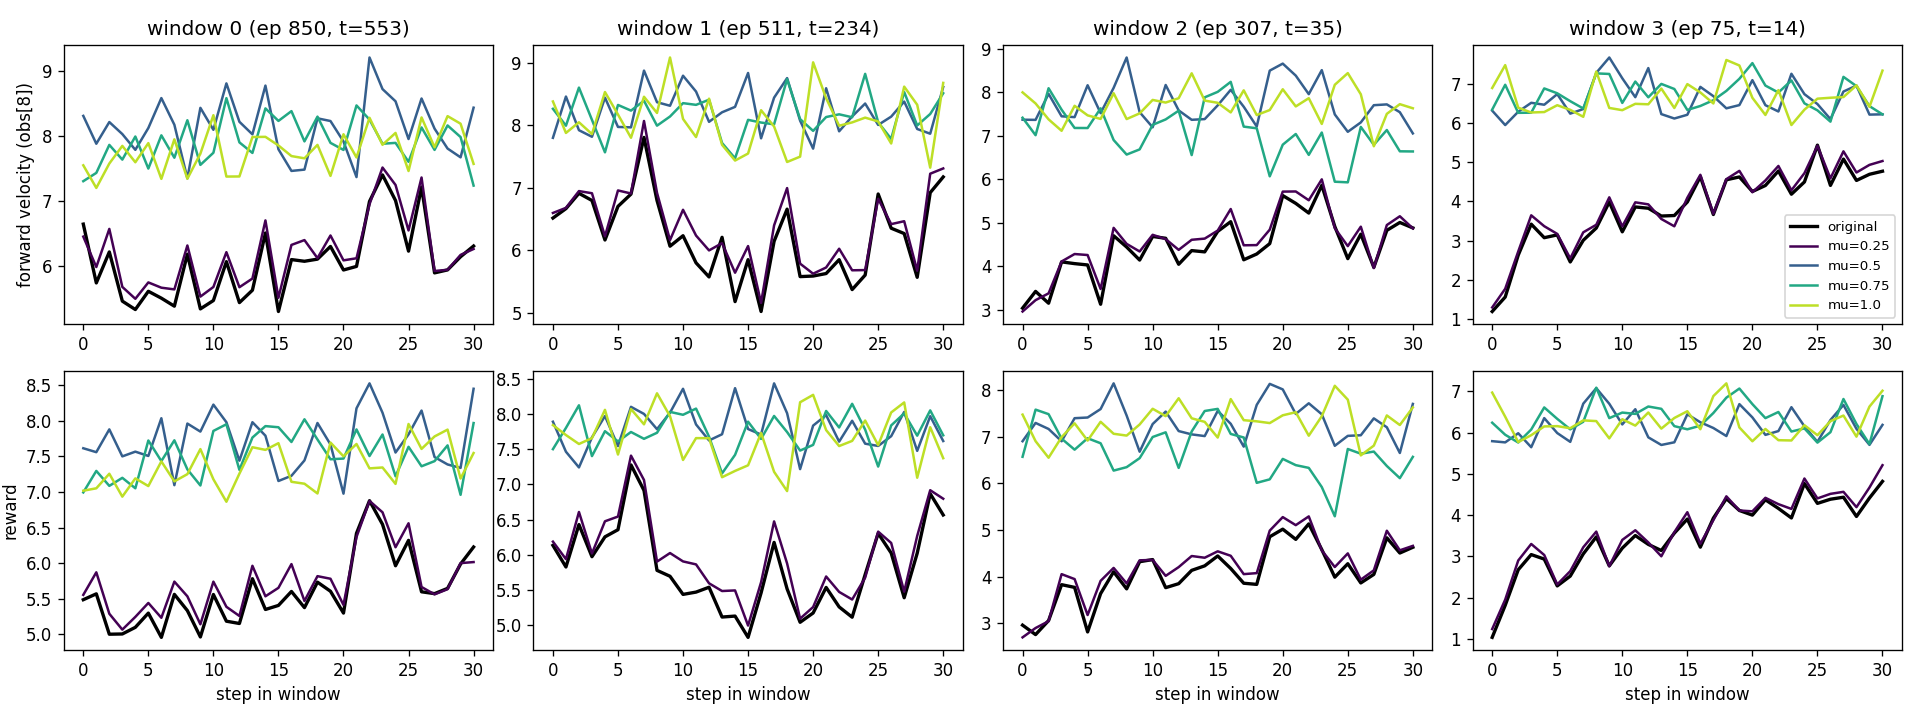
\includegraphics[width=\linewidth]{demo_mu_sweep.png}

\scriptsize Top: forward velocity \texttt{s[8]}; bottom: reward, over the 31 steps. Black = original.
\end{column}
\begin{column}{0.44\linewidth}
\scriptsize
\begin{tabular}{lrrrr}
\toprule
win & $\mu$ & $R_{\text{sim}}$ & dyn MSE & shift\\
\midrule
0 & 0 & 173.5 & -- & 0\\
0 & 0.25 & 177.6 & 0.0011 & 0.13\\
0 & 0.5 & 239.1 & 0.0063 & 0.84\\
0 & 1.0 & 227.8 & 0.0064 & 1.31\\
3 & 0 & 109.4 & -- & 0\\
3 & 0.25 & 112.9 & 0.0114 & 0.14\\
3 & 0.5 & 191.0 & 0.0021 & 1.04\\
3 & 1.0 & 194.1 & 0.0019 & 1.49\\
\bottomrule
\end{tabular}

\vspace{0.4em}
\begin{itemize}
\item $\mu=0.25$: almost no change ($+3\%$ reward).
\item $\mu\ge0.5$: $+35$--$75\%$ reward; model reward matches the simulator within 0.5.
\item Columns defined on the next slides.
\end{itemize}
\end{column}
\end{columns}
\end{frame}

% =============================================================================================
\section{Making H2 measurable}
\begin{frame}{Unit of analysis and quality $Q$}
\textbf{Unit:} one source window $i$ (31 transitions + final state), identified by (episode, start).
\vspace{0.4em}

\textbf{Eligible windows (H2 study):} starts $0,\dots,800$ of every episode $\Rightarrow 801\times1000=$ \textbf{801{,}000}.
Later starts are excluded because their RTG (the conditioning value) is cut short by the episode end.
\vspace{0.6em}

\textbf{Quality} = discounted reward inside the window:
\[
q_i=\sum_{t=0}^{30}0.99^{\,t}\,r_{\text{start}_i+t},\qquad Q_i=\text{percentile rank of }q_i\text{ in the pool}\in(0,1].
\]
\begin{itemize}
\item Inside-the-window reward is used instead of RTG because RTG falls for late windows regardless of behaviour.
\item RTG is still what the model is conditioned on (step 2 of the edit).
\end{itemize}
\end{frame}

\begin{frame}{Local support $S_1$: nearest neighbours in the data (model-free)}
\begin{enumerate}
\item Standardise every $(s,a)\in\mathbb R^{23}$: $z=(x-\bar x)/\mathrm{sd}(x)$ over all 1M transitions.
\item For each step $t$ of window $i$ (global transition $j_t$): distance to the \textbf{20th nearest} transition from a \textbf{different episode},
\[
d_{20}(j_t)=\text{20th smallest of }\{\lVert z_{j_t}-z_{j'}\rVert_2:\ \text{episode}(j')\neq\text{episode}(j_t)\}.
\]
Same-episode neighbours are excluded: adjacent steps of one run are always near-identical.
\item $\text{s1\_dist}_i=\operatorname{median}_t\,d_{20}(j_t)$; \quad $S_{1,i}=$ percentile rank of $-\text{s1\_dist}_i$.
\end{enumerate}
\vspace{0.4em}
\textbf{Why it measures density:} the $k$-NN estimate $\hat p(x)=k/(N\,V_d\,d_k(x)^d)$ ($d=23$): smaller $d_{20}$ $\Leftrightarrow$ denser region.
It is the inverse of GTA's own \emph{novelty} metric (paper Eq.~12).
\vspace{0.3em}

\small Exact brute force (FAISS on CPU, or PyTorch on GPU; identical to $10^{-5}$).
\end{frame}

\begin{frame}{Local support $S_2$: how well the trained model reconstructs the window}
\begin{enumerate}
\item Normalise the window: $\tilde x$. For $\sigma\in\{0.16,\,0.5,\,2.4\}$ and 4 draws $\varepsilon_n\sim\mathcal N(0,I)$, one \emph{unconditional} denoiser call
\[
\hat x=D_\theta(\tilde x+\sigma\varepsilon_n;\sigma,\varnothing),\qquad
D_\theta(x;\sigma)=c_{\text{skip}}x+c_{\text{out}}F_\theta(c_{\text{in}}x;c_{\text{noise}})
\]
with $c_{\text{skip}}=\frac{1}{\sigma^2+1}$, $c_{\text{out}}=\frac{\sigma}{\sqrt{\sigma^2+1}}$, $c_{\text{in}}=\frac{1}{\sqrt{\sigma^2+1}}$, $c_{\text{noise}}=\tfrac14\ln\sigma$.
\item Error $e_i(\sigma)=\frac14\sum_n \frac{\sum_{t,d}M_{td}(\hat x-\tilde x)^2_{td}}{\sum M}$ (mask $M$ drops row 31's action/reward zeros, as in training).
\item $\text{s2\_score}_i=-\operatorname{mean}_\sigma\, z\text{-score}_{\text{pool}}\big(\ln e_i(\sigma)\big)$; \quad $S_{2,i}=$ percentile rank.
\end{enumerate}
\vspace{0.3em}
\textbf{Why:} $-\log p(x)\le\int w(\sigma)\,\mathbb E_\varepsilon\lVert D_\theta(x+\sigma\varepsilon;\sigma)-x\rVert^2d\sigma+C$ (Kingma et al.\ 2021; Song et al.\ 2021). $S_2$ is a 3-point version.
The three $\sigma$ are the noise levels an edit applies at $\mu\approx0.25,\,0.35,\,0.5$.
\textbf{$S_2$ is the primary support metric.}
\end{frame}

\begin{frame}{Local support $S_3$ (validation only) and agreement of the three}
\small
\textbf{$S_3$: exact log-likelihood} via the probability-flow ODE $\frac{dx}{d\sigma}=f(x,\sigma)=\frac{x-D_\theta(x;\sigma)}{\sigma}$:
\[
\log p_0(x)=\log\mathcal N(x_{\sigma_{\max}};0,\sigma_{\max}^2I)+\int_{\sigma_{\min}}^{\sigma_{\max}}\nabla\!\cdot f(x_\sigma,\sigma)\,d\sigma,
\]
divergence by Hutchinson ($v^\top\partial_xf\,v$, one Rademacher probe), dopri5, tol $10^{-4}$. Slow: computed on \textbf{100} pool windows.
\vspace{0.5em}

\begin{columns}[T]
\begin{column}{0.45\linewidth}
\centering
\begin{tabular}{lr}
\toprule
pair (pool, $n=20{,}000$) & Spearman $\rho$\\
\midrule
$S_1$ vs $S_2$ & 0.79\\
$S_2$ vs $S_3$ ($n=100$) & 0.74\\
$S_1$ vs $S_3$ ($n=100$) & 0.83\\
$Q$ vs $S_1$ & 0.49\\
$Q$ vs $S_2$ & 0.42\\
\bottomrule
\end{tabular}
\end{column}
\begin{column}{0.53\linewidth}
\begin{itemize}
\item Data-based and model-based support agree; both track the exact likelihood.
\item Support and quality are related but not the same (needed for a 2-D design).
\item Support spread: $(p_{90}-p_{10})/\text{median}$ of s1\_dist $=0.52$.
\end{itemize}
\end{column}
\end{columns}
\end{frame}

\begin{frame}{What is measured for every edit}
Each edited window $\hat\tau$ is replayed in MuJoCo: for each of the 31 rows, set the simulator to $\hat s_t$ (x-position $:=0$, unobserved and irrelevant to dynamics), apply $\hat a_t$, read the true next state $f^*(\hat s_t,\hat a_t)$ and true reward.
\vspace{0.4em}

\small
\begin{tabularx}{\linewidth}{lY}
\toprule
\texttt{gen\_r} & $\sum_t\hat r_t$: sum of the 31 rewards \emph{written by the model}\\
\texttt{oracle\_r} & $\sum_t r_{\text{env}}(\hat s_t,\hat a_t)$: the \emph{true} reward of the edited states/actions (paper App.~D.3)\\
\texttt{src\_oracle\_r} & the same for the unedited source window\\
\texttt{gain\_rel} & $(\texttt{oracle\_r}-\texttt{src\_oracle\_r})/\max(|\texttt{src\_oracle\_r}|,1)$: relative reward gain\\
\texttt{dyn\_mse} & $\frac{1}{31\cdot17}\sum_{t,d}\big((f^*(\hat s_t,\hat a_t)-\hat s_{t+1})_d/\mathrm{sd}_d\big)^2$: physics error, dataset-std units (paper Eq.~11)\\
\texttt{shift} & $\sqrt{\frac{1}{31\cdot17}\sum_{t,d}((\hat s_t-s_t)_d/\mathrm{sd}_d)^2}$: how far the edit moved from the source\\
\bottomrule
\end{tabularx}
\vspace{0.3em}

Every (window, $\mu$) is edited \textbf{twice} (two noise draws); metrics are averaged over the draws.
\end{frame}

\begin{frame}{From edits to ``the best $\mu$'' of a window}
\small
For window $i$ with metrics $\text{gain}_i(\mu)$, $\text{dyn}_i(\mu)$ on the grid $\mathcal M$ and threshold $\theta$:
\begin{itemize}
\item $\mu^*_i=\arg\max\{\text{gain}_i(\mu):\ \mu\in\mathcal M,\ \text{dyn}_i(\mu)\le\theta\}$ \hfill best reward among physically valid edits
\item $\mu_{90,i}=\min\{\mu:\ \text{gain}_i(\mu)\ge0.9\,\max_{\mu'}\text{gain}_i(\mu')\}$ \hfill how much editing the window needs
\item $\mu^{\text{safe}}_i=$ largest $\mu$ before $\text{dyn}_i$ first exceeds $\theta$ (0 if already at $\mu=0.1$) \hfill how far it can be pushed safely
\end{itemize}
\textbf{Statistics} (per outcome $y\in\{\mu^*,\mu_{90},\mu^{\text{safe}}\}$, $n=400$):
\[
y_i=\beta_0+\beta_Q(Q_i-\tfrac12)+\beta_S(S_i-\tfrac12)+\beta_{QS}(Q_i-\tfrac12)(S_i-\tfrac12)+e_i
\]
$\beta_S$ = change of $y$ from the least to the best supported window (quality fixed). 95\% CI: 2{,}000 bootstrap resamples of windows. $p$: 2{,}000 permutations of $S$ (or $Q$).
\vspace{0.3em}

\textbf{Decision rule (fixed before the main run):} \yes{} if CI($\beta_S$)$>0$, CI($\beta_Q$)$<0$ \emph{and} $\bar y(\text{low }Q,\text{high }S)-\bar y(\text{high }Q,\text{low }S)\ge0.1$; partly if only one effect.
\end{frame}

% =============================================================================================
\section{Pilot}
\begin{frame}{Pilot study: design}
\small
\begin{tabularx}{\linewidth}{lY}
\toprule
Pool & 500 random eligible windows (seed 1), support $S_1$ only (kNN)\\
Sample & $5\times5$ grid on ($Q$ quintile $\times$ $S_1$ quintile), up to 8 per cell $\Rightarrow$ \textbf{184 windows} (the low-$Q$/high-$S$ corner was under-filled)\\
$\mu$ grid & 0.1, 0.2, 0.3, 0.35, 0.4, 0.45, 0.5, 0.75; 2 draws each $\Rightarrow$ 2{,}944 edits\\
Runtime & 36 s on the GPU\\
Purpose & check the pipeline and the outcome definitions before the main run\\
\bottomrule
\end{tabularx}
\vspace{0.3em}

\centering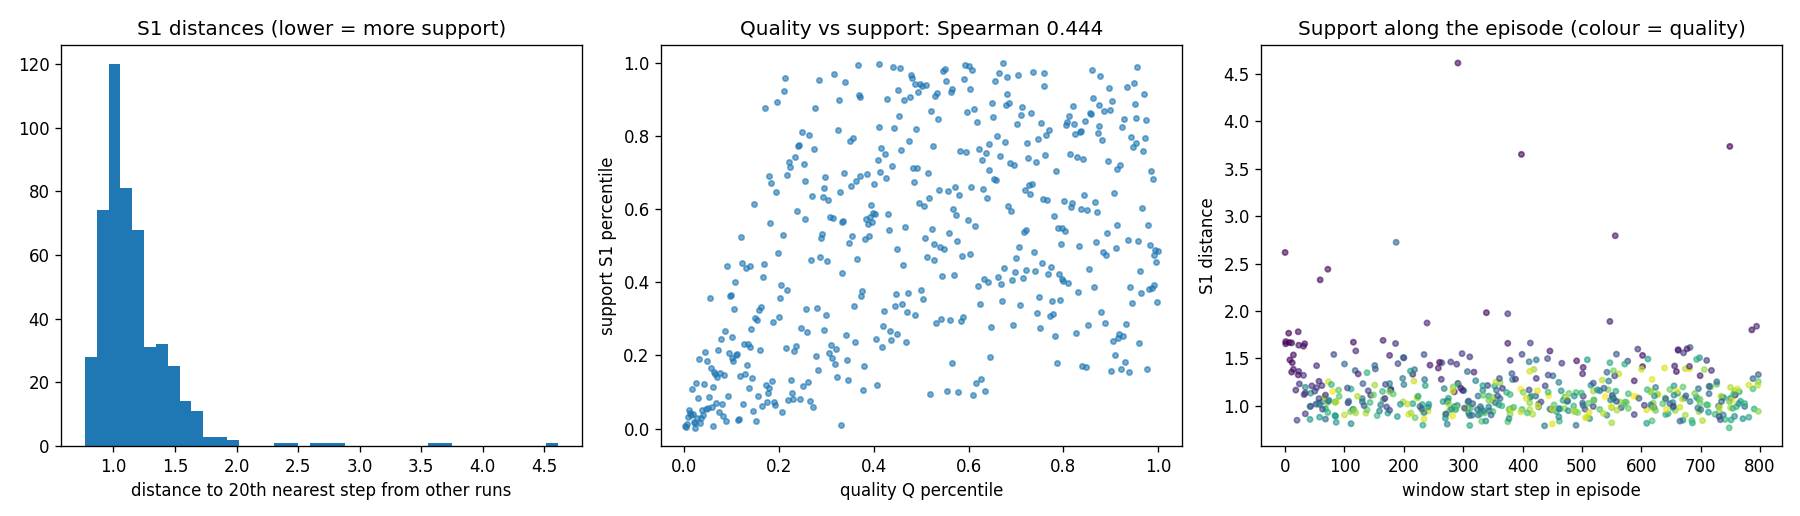
\includegraphics[width=0.85\linewidth]{pilot_knn_preview.png}

\raggedright

\scriptsize 500 windows. Left: $S_1$ distances (median 1.09, $p_{10}$/$p_{90}$ 0.90/1.49). Middle: low-quality windows almost always have low support (Spearman 0.44). Right: least-supported windows are episode starts (the cheetah accelerating from rest).
\end{frame}

\begin{frame}{Pilot results: the first definition was dominated by a ceiling effect}
\begin{columns}[T]
\begin{column}{0.42\linewidth}
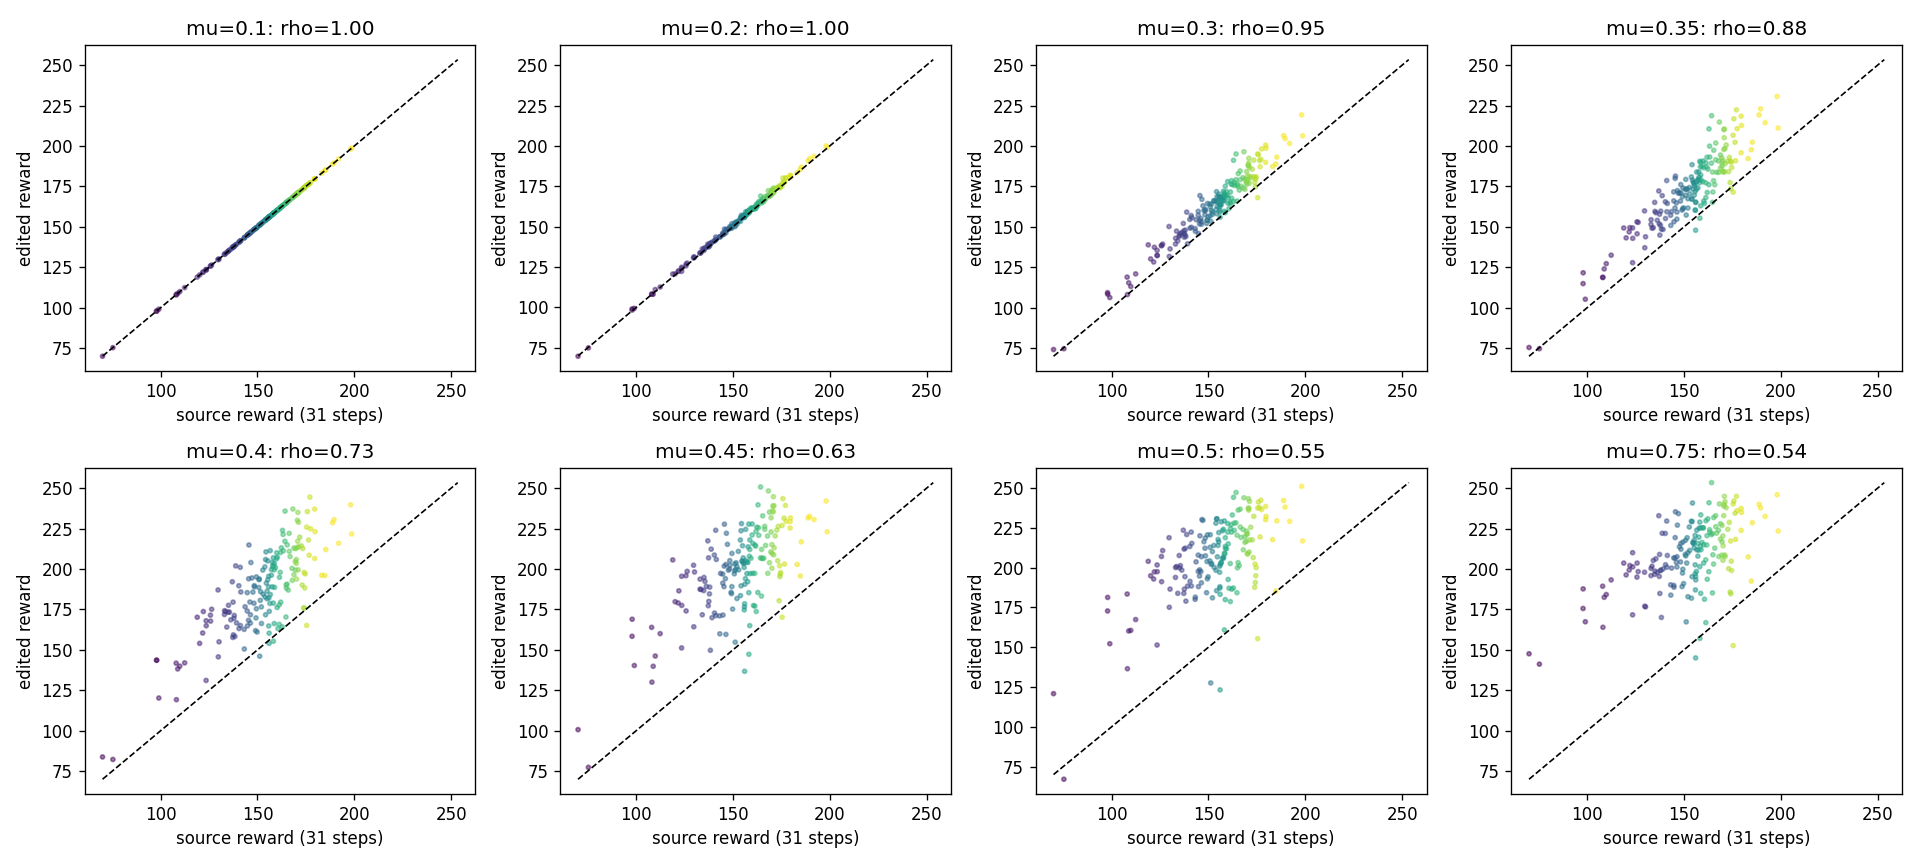
\includegraphics[width=\linewidth]{pilot_ceiling.png}

\scriptsize Edited vs source reward per $\mu$ (184 windows). At $\mu\ge0.45$ edits converge to $\approx175$--$250$ whatever the source: rank correlation falls from 1.00 to 0.54.
\end{column}
\begin{column}{0.56\linewidth}
\scriptsize
\begin{tabular}{@{}lll@{}}
\toprule
$\mu^*$ analysed with & $\beta_Q$ [95\% CI] & $\beta_S$ [95\% CI]\\
\midrule
all $\mu$, $\theta=0.017$ & $-0.17$ $[-0.24,-0.10]$ & $+0.02$ $[-0.05,0.09]$\\
all $\mu$, $\theta=0.0085$ & $-0.15$ $[-0.22,-0.08]$ & $-0.01$ $[-0.08,0.07]$\\
$\mu\le0.5$, $\theta=0.017$ & $-0.02$ $[-0.05,0.00]$ & $+0.01$ $[-0.02,0.05]$\\
$\mu\le0.5$, $\theta=0.0085$ & $-0.01$ $[-0.05,0.02]$ & $\mathbf{+0.09}$ $[0.04,0.14]$\\
\bottomrule
\end{tabular}
\vspace{0.5em}
\begin{itemize}
\item The apparent quality effect came from $\mu=0.75$ edits that rewrite every window to a similar high reward.
\item Restricting to $\mu\le0.5$ (edits that keep part of the source) removes it and reveals a support effect.
\item \textbf{Fixed for the main run:} $\mu\le0.5$, $\theta=0.0085$ (paper's mean dynamic MSE, Table~19), support $S_2$.
\end{itemize}
\end{column}
\end{columns}
\end{frame}

% =============================================================================================
\section{Main study}
\begin{frame}{Main study: which part of the data is used (funnel)}
\centering\small
\begin{tabular}{@{}lrl@{}}
\toprule
stage & count & how\\
\midrule
transitions in the dataset & 1{,}000{,}000 & 1{,}000 episodes $\times$ 1{,}000\\
windows (all starts) & 970{,}000 & 970 per episode\\
eligible windows (start $\le800$) & 801{,}000 & H2 study only\\
pool & 20{,}000 & uniform random, seed 0; $Q$, $S_1$, $S_2$ computed\\
\quad of which with $S_3$ & 100 & random subset\\
selected windows & \textbf{400} & $5\times5$ grid on $Q\times S_2$ quintiles, 16 per cell\\
edits generated & 6{,}400 & $400\times8\ \mu\times2$ draws\\
edits analysed & \textbf{5{,}600} & $400\times7\ \mu\ (\le0.5)\times2$ draws\\
simulated transitions & 198{,}400 & $6{,}400\times31$ MuJoCo steps\\
\bottomrule
\end{tabular}
\vspace{0.6em}

\raggedright\small Settings: $\alpha=1.3$, temperature 1, threshold $\theta=0.0085$, $\mu\in\{0.1,0.2,0.3,0.35,0.4,0.45,0.5\}$.
\end{frame}

\begin{frame}{The pool: quality and support distributions}
\centering
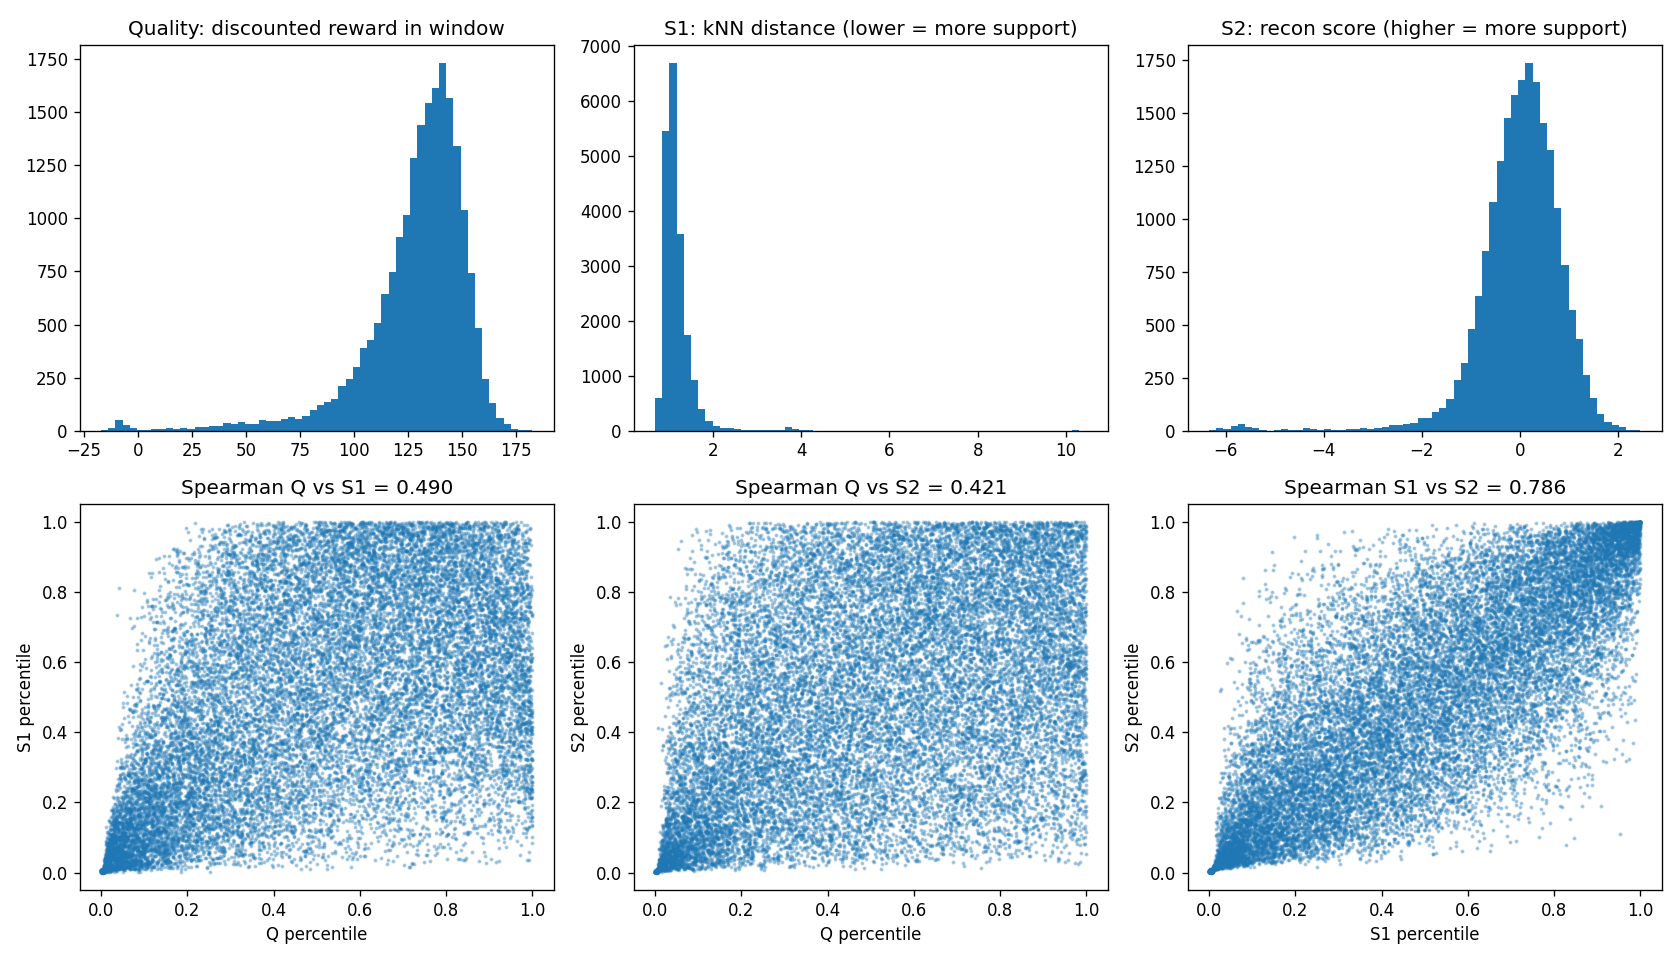
\includegraphics[width=0.82\linewidth]{main_pool_overview.png}

\raggedright\scriptsize Top: histograms of $q$, s1\_dist, s2\_score. Bottom: pairwise percentile scatter with Spearman $\rho$ (20{,}000 windows). Low-quality windows are rarely well supported, which is why sampling is stratified on both axes.
\end{frame}

\begin{frame}{Main result 1: what changes with $\mu$, by quadrant}
\centering
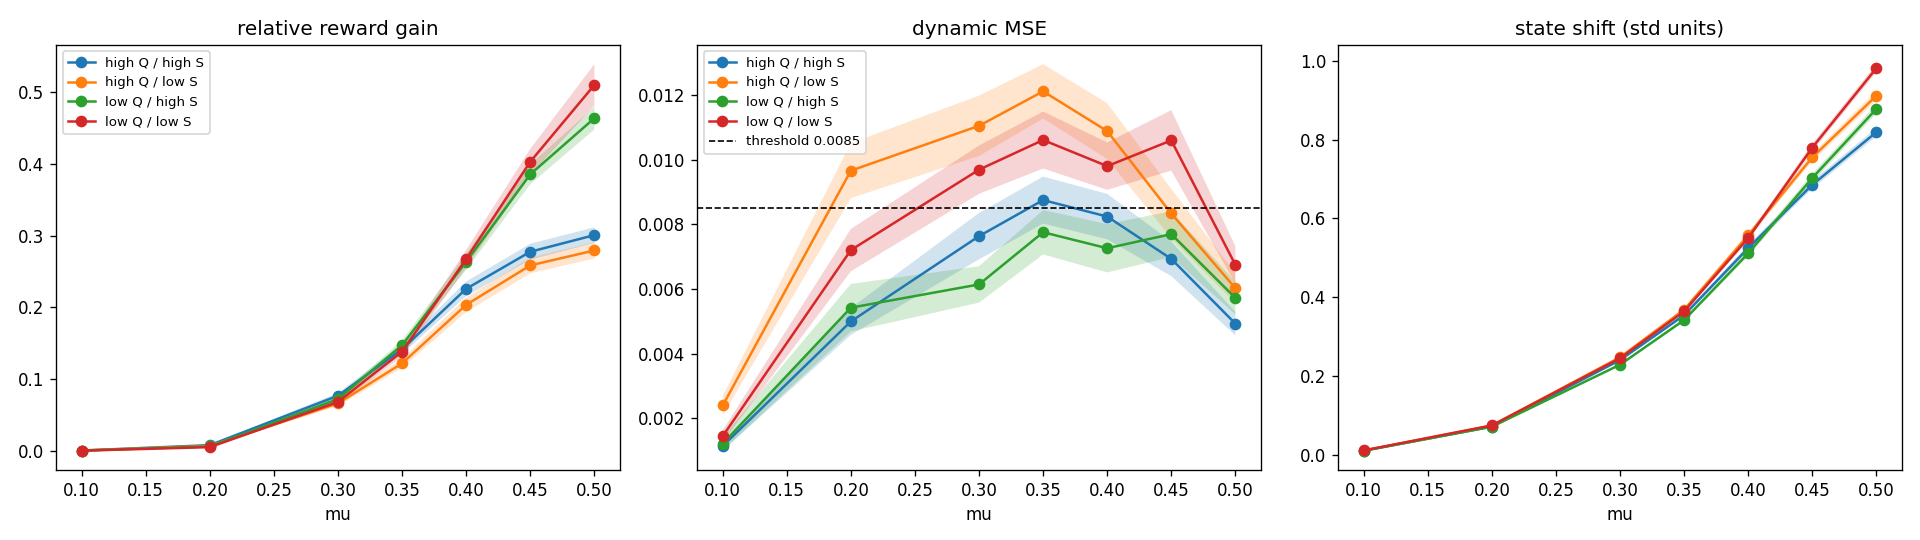
\includegraphics[width=\linewidth]{main_quadrant_curves.png}

\raggedright\small
Quadrants split $Q$ and $S_2$ at their medians ($\approx$100 windows each); bands $=\pm1$ s.e.
\begin{itemize}
\item \textbf{Reward gain} (left) rises with $\mu$ for everyone; low-$Q$ windows gain most.
\item \textbf{Physics error} (middle) is higher for \emph{low-support} windows (orange, red) at every $\mu$; it peaks at $\mu\approx0.35$ and falls at 0.5.
\item \textbf{Shift} (right) is the same for all quadrants: equal edit size, unequal damage.
\end{itemize}
\end{frame}

\begin{frame}{Main result 2: gain follows quality, physics error follows support}
\centering
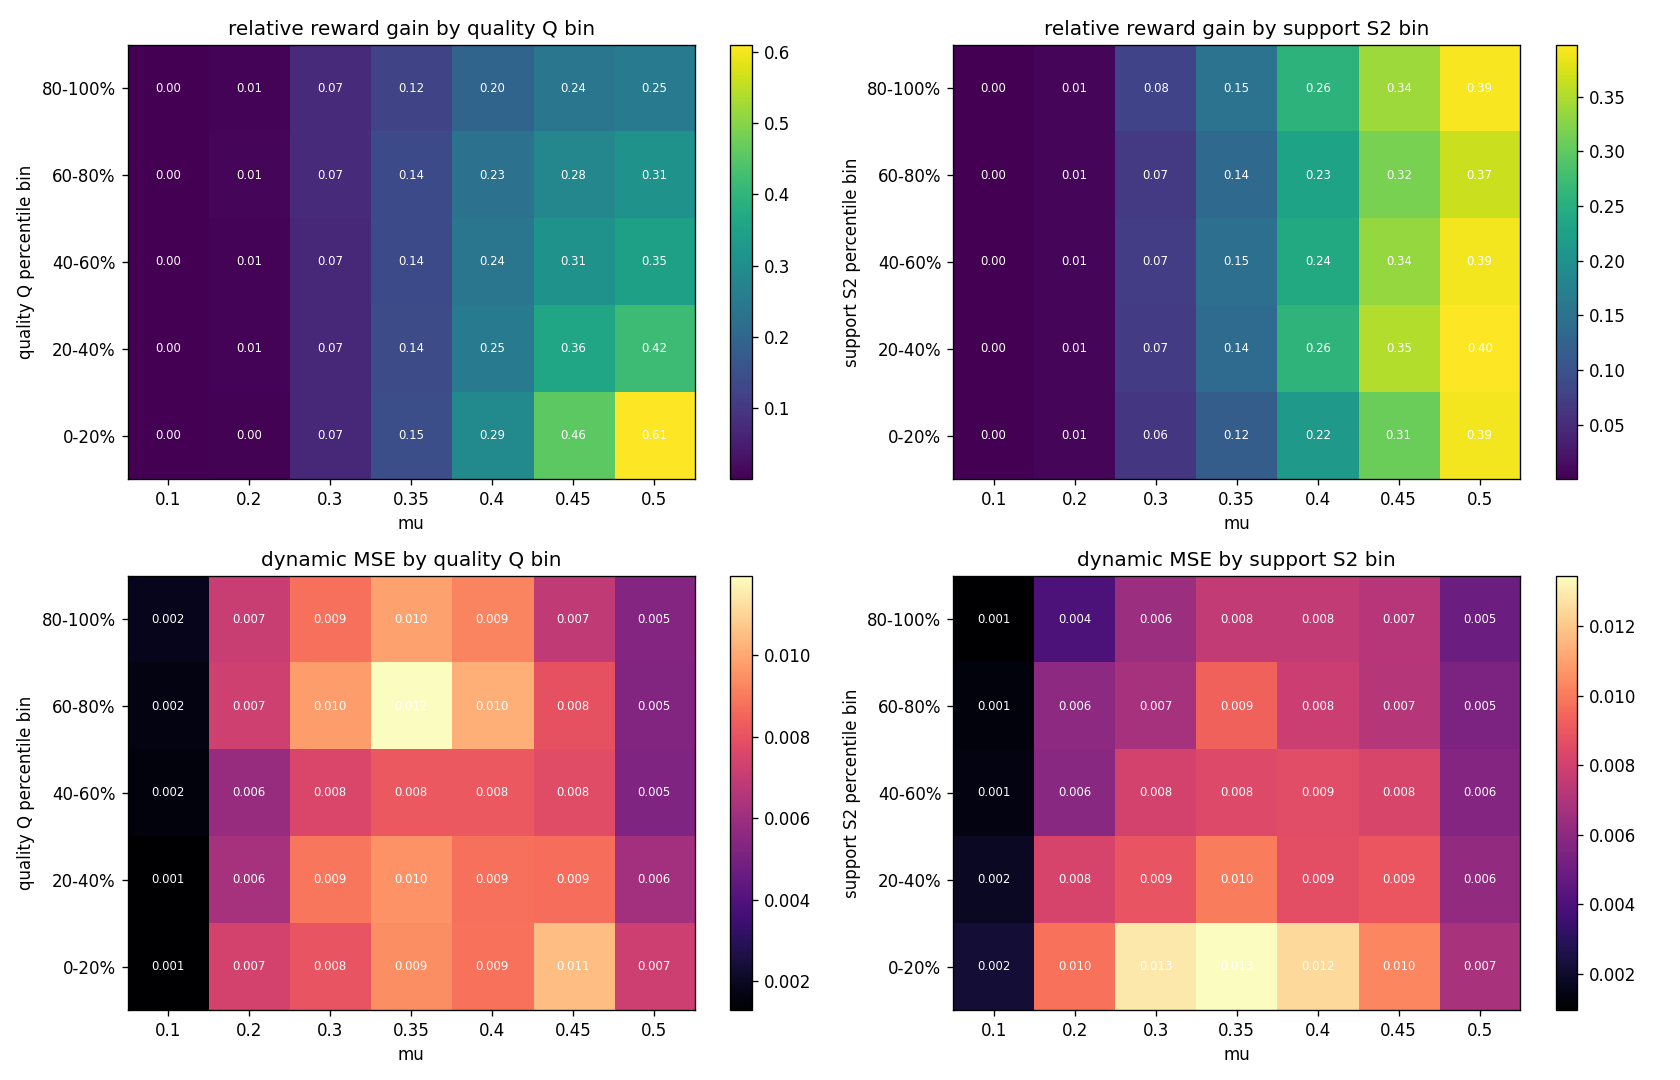
\includegraphics[width=0.7\linewidth]{main_heatmaps.png}

\raggedright\scriptsize Rows: percentile bins (80 windows each); columns: $\mu$. Top-left: lowest-quality bin gains $+61\%$ at $\mu=0.5$, highest $+25\%$. Bottom-right: lowest-support bin reaches dynamic MSE 0.012--0.013 at $\mu=0.3$--$0.4$, highest-support bin 0.006--0.008 ($\approx2\times$).
\end{frame}

\begin{frame}{Main result 3: correlations at every $\mu$ (Spearman, 400 windows)}
\centering
\small
\begin{tabular}{lrrrrrrr}
\toprule
$\mu$ & 0.1 & 0.2 & 0.3 & 0.35 & 0.4 & 0.45 & 0.5\\
\midrule
$S_2$ vs physics error & $-0.29$ & $-0.36$ & $-0.34$ & $-0.28$ & $-0.24$ & $-0.18$ & $-0.13$\\
$S_1$ vs physics error & $-0.25$ & $-0.34$ & $-0.32$ & $-0.26$ & $-0.28$ & $-0.25$ & $-0.15$\\
$Q$ vs physics error & $+0.07$ & $+0.01$ & $+0.01$ & $+0.09$ & $+0.04$ & $-0.14$ & $-0.07$\\
\midrule
$S_2$ vs reward gain & $+0.11$ & $+0.11$ & $+0.12$ & $+0.14$ & $+0.09$ & $+0.06$ & $+0.06$\\
$Q$ vs reward gain & $+0.13$ & $+0.17$ & $+0.01$ & $-0.11$ & $-0.25$ & $-0.51$ & $-0.65$\\
\midrule
mean reward gain & 0.000 & 0.007 & 0.071 & 0.138 & 0.240 & 0.331 & 0.388\\
mean physics error & 0.0015 & 0.0068 & 0.0086 & 0.0098 & 0.0090 & 0.0084 & 0.0058\\
share over $\theta=0.0085$ & 0.02 & 0.24 & 0.36 & 0.43 & 0.41 & 0.33 & 0.18\\
\bottomrule
\end{tabular}
\vspace{0.6em}

\raggedright
\begin{itemize}
\item Both support metrics predict physics error at every $\mu$; quality does not (mechanism of H2a).
\item Quality predicts reward gain (ceiling effect: edits converge towards similar reward).
\end{itemize}
\end{frame}

\begin{frame}{Main result 3 (visual): support vs physics error per $\mu$}
\centering
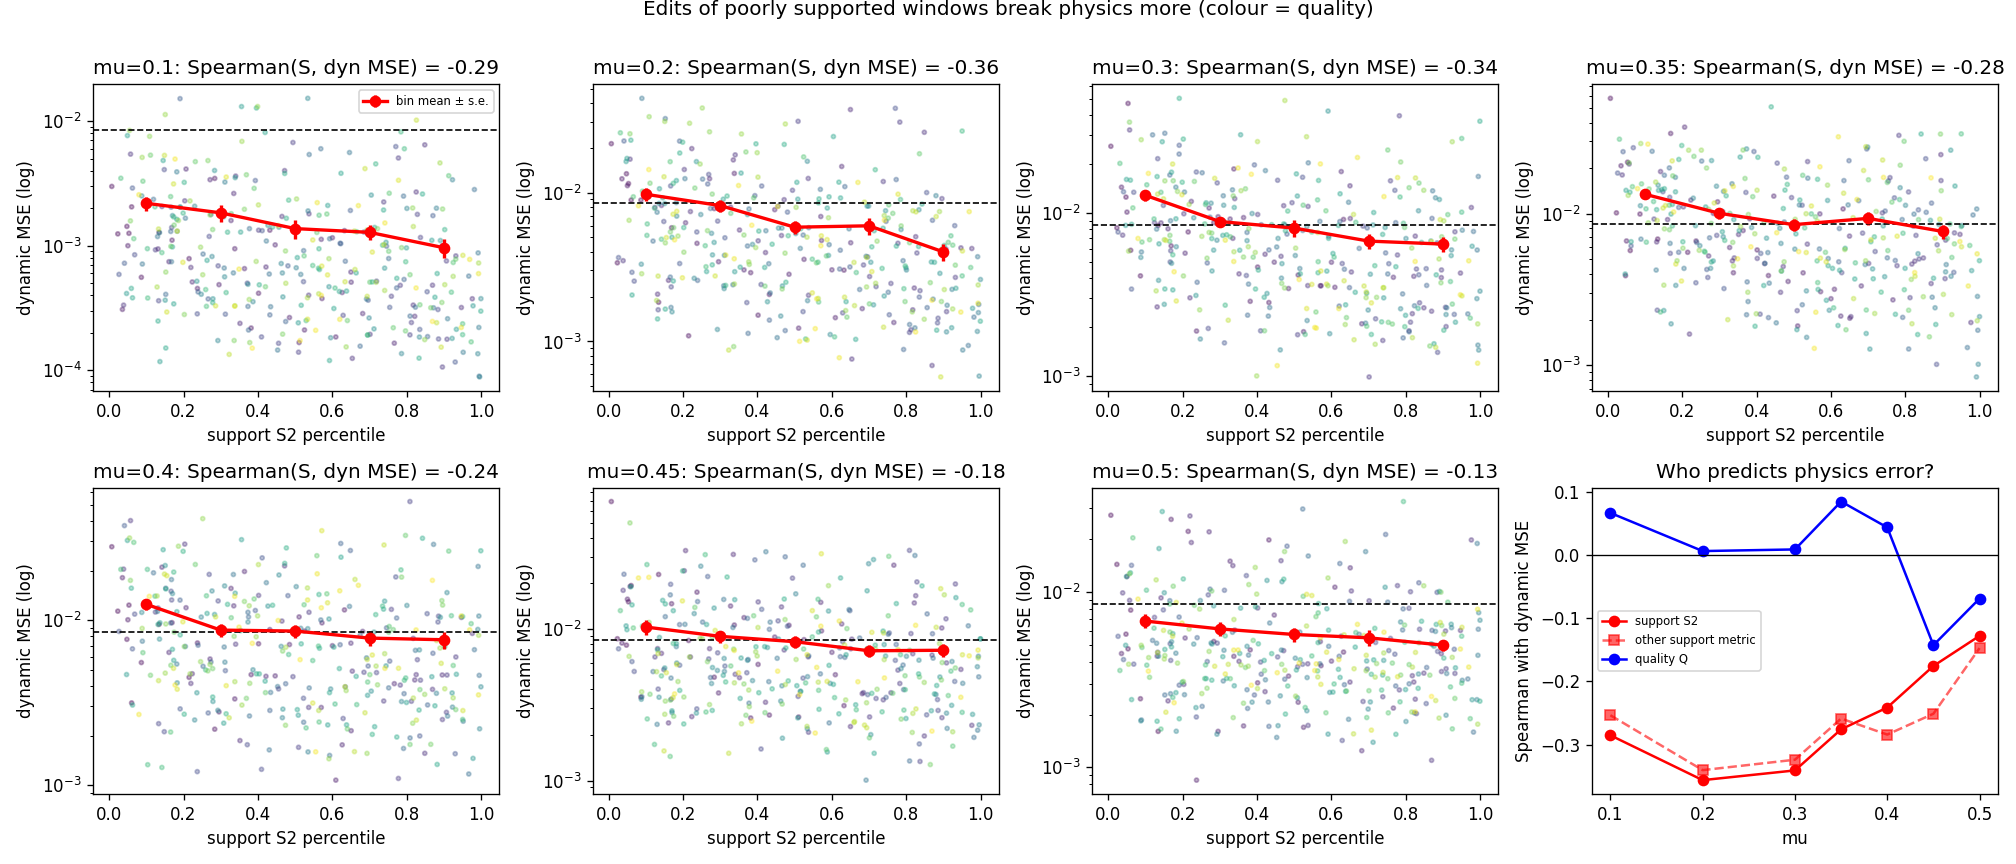
\includegraphics[width=\linewidth]{main_support_vs_physics.png}

\raggedright\scriptsize Each dot = one window (colour = quality); red = mean $\pm$ s.e.\ per support quintile; dashed = $\theta$; log scale. Last panel: correlation of physics error with $S_2$ (solid), $S_1$ (dashed) and $Q$ (blue) across $\mu$.
\end{frame}

\begin{frame}{Main result 4: test of H2 (decision rule fixed in advance)}
\centering
\footnotesize
\begin{tabular}{@{}llllll@{}}
\toprule
outcome & $\beta_S$ [95\% CI] & $p_S$ & $\beta_Q$ [95\% CI] & gap & verdict\\
\midrule
$\mu^*$ & $+0.059$ $[0.030,0.090]$ & $<0.001$ & $-0.001$ $[-0.025,0.022]$ & $+0.034$ & S only, small\\
$\mu_{90}$ & $-0.002$ $[-0.014,0.009]$ & 0.78 & $-0.048$ $[-0.063,-0.034]$ & $+0.020$ & Q only, small\\
$\mu^{\text{safe}}$ $^\dagger$ & $\mathbf{+0.183}$ $[0.139,0.225]$ & $<0.001$ & $-0.013$ $[-0.061,0.036]$ & $\mathbf{+0.109}$ & S only\\
\bottomrule
\end{tabular}
\vspace{0.4em}

\raggedright\footnotesize
All three verdicts are ``partly supported''. gap $=\bar y(\text{low }Q/\text{high }S)-\bar y(\text{high }Q/\text{low }S)$ (rule needs $\ge0.1$). $\beta_{QS}$ not significant for any outcome.
$^\dagger$ $\mu^{\text{safe}}$ was defined after the first look at this run (exploratory); at $\theta=0.017$ it gives $\beta_S=+0.110$ $[0.062,0.155]$, $\beta_Q=-0.030$ $[-0.075,0.014]$.
\vspace{0.4em}

\small
\textbf{Why $\mu^*$ moves so little:} reward keeps rising up to the top of the grid, so the best valid $\mu$ is usually the largest:
\begin{center}
\begin{tabular}{lrrrrrrr}
\toprule
$\mu^*$ & 0.1 & 0.2 & 0.3 & 0.35 & 0.4 & 0.45 & 0.5\\
windows & 9 & 2 & 6 & 5 & 13 & 86 & \textbf{279}\\
\bottomrule
\end{tabular}
\end{center}
\end{frame}

\begin{frame}{Main result 5: how far can a window be edited safely?}
\centering
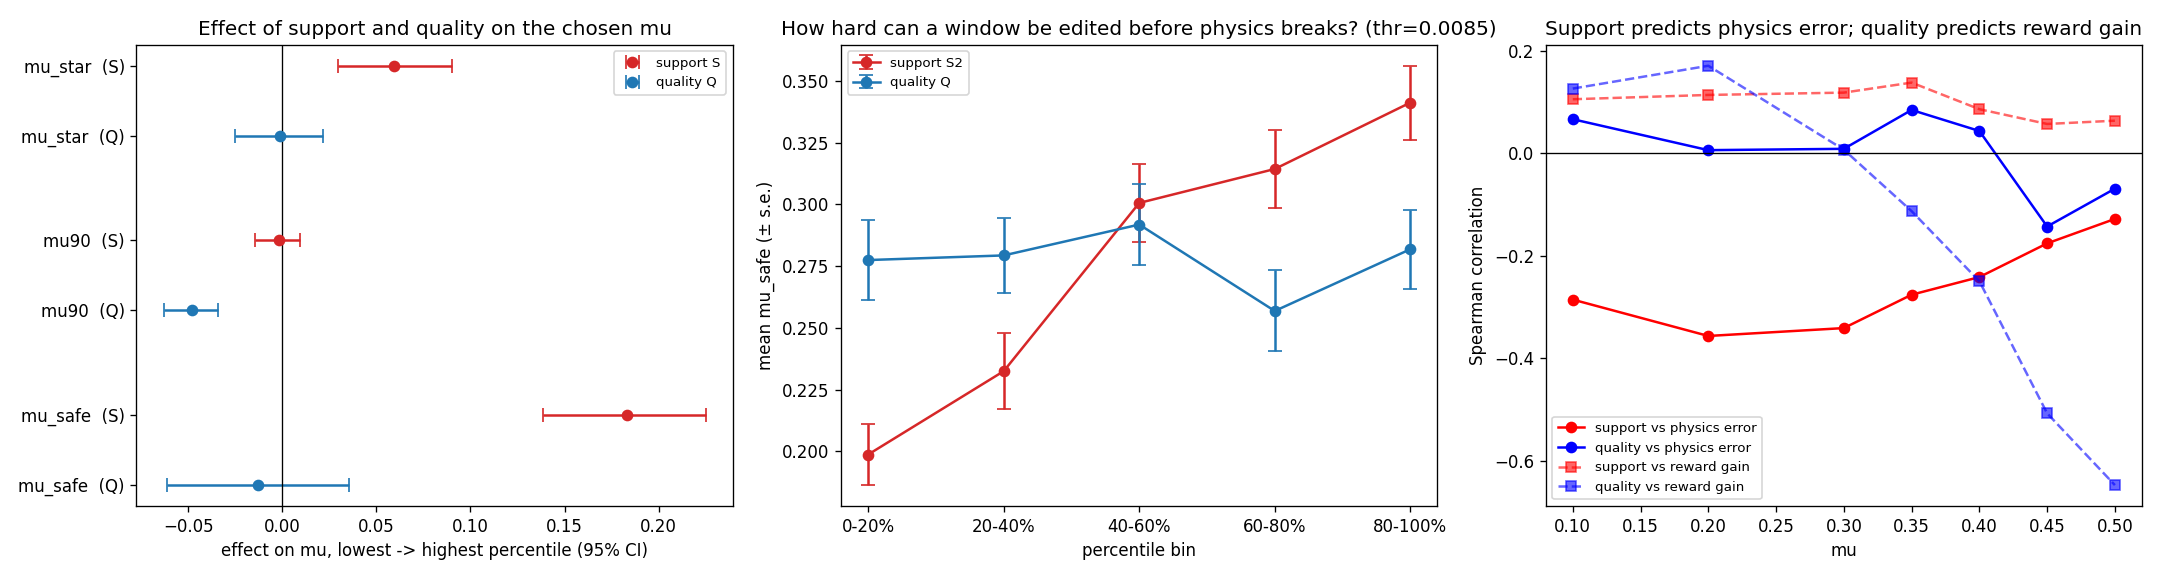
\includegraphics[width=\linewidth]{main_correlation_summary.png}

\raggedright\small
\begin{itemize}
\item Left: effects on each outcome; support (red) is right of zero for $\mu^*$ and $\mu^{\text{safe}}$, quality (blue) is not below zero except a small $\mu_{90}$ effect.
\item Middle: mean $\mu^{\text{safe}}$ by support quintile \textbf{0.20, 0.23, 0.30, 0.31, 0.34}; by quality quintile flat at $\approx0.26$--$0.29$.
\item Right: support predicts physics error, quality predicts reward gain.
\end{itemize}
\end{frame}

\begin{frame}{Main result 6: best-$\mu$ maps over the $5\times5$ design}
\centering
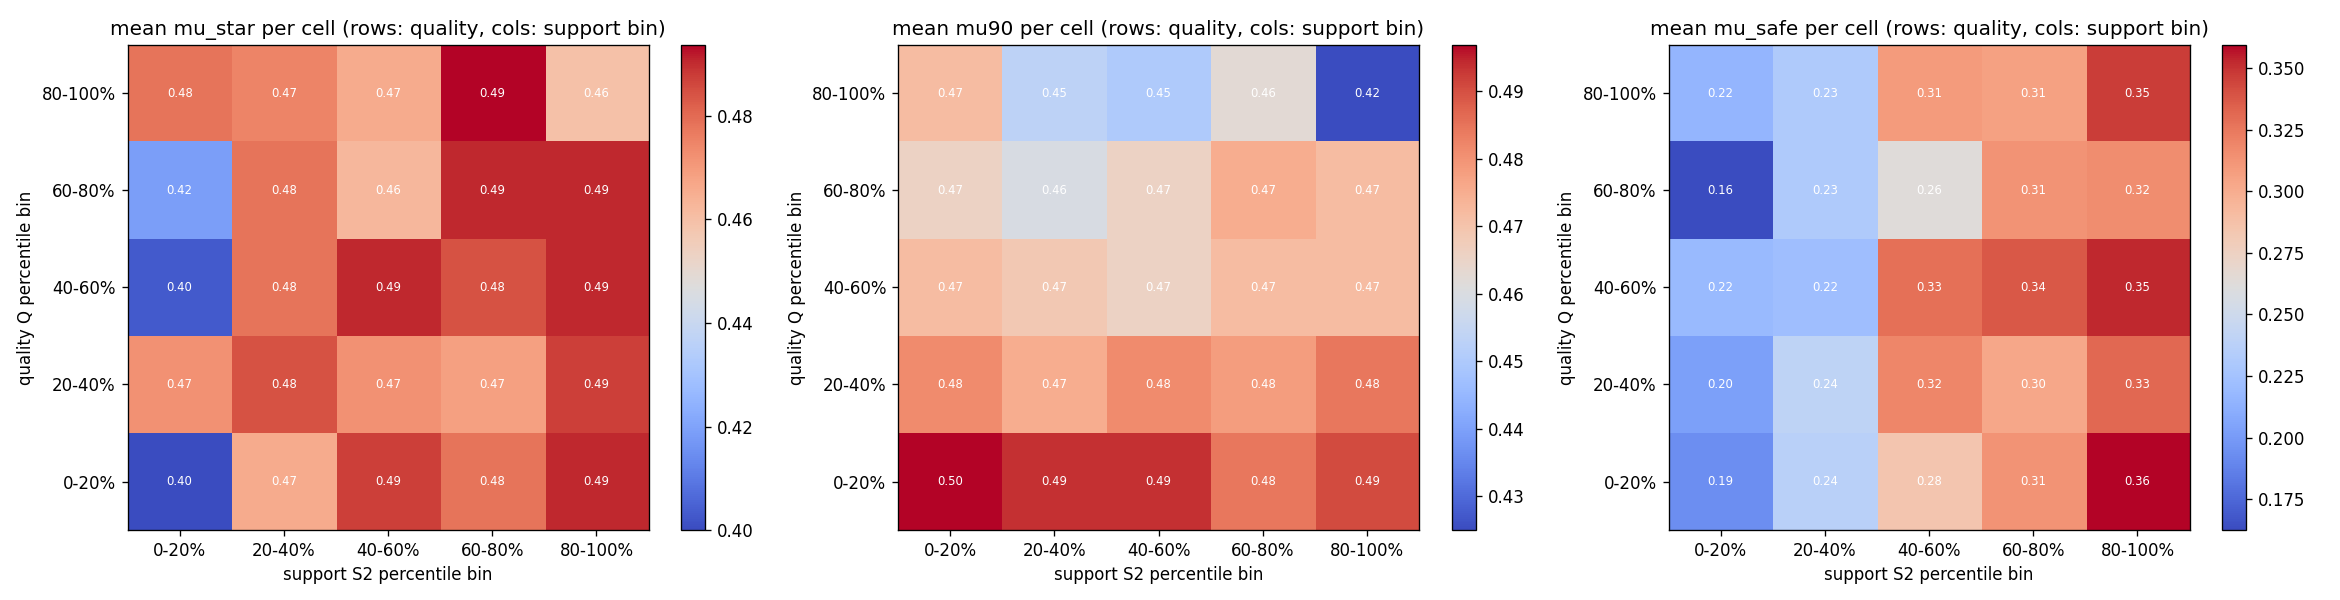
\includegraphics[width=\linewidth]{main_best_mu_map.png}

\raggedright\small
Each cell = mean over its 16 windows. Rows: quality quintile; columns: support quintile.
\begin{itemize}
\item $\mu^*$ (left) $\approx0.47$--$0.49$ almost everywhere: pinned at the top of the grid.
\item $\mu^{\text{safe}}$ (right) goes from blue ($\approx0.16$--$0.24$) in low-support columns to red ($\approx0.31$--$0.36$) in high-support columns \textbf{in every quality row}.
\end{itemize}
\end{frame}

\begin{frame}{Check: the ceiling effect in the main run}
\centering
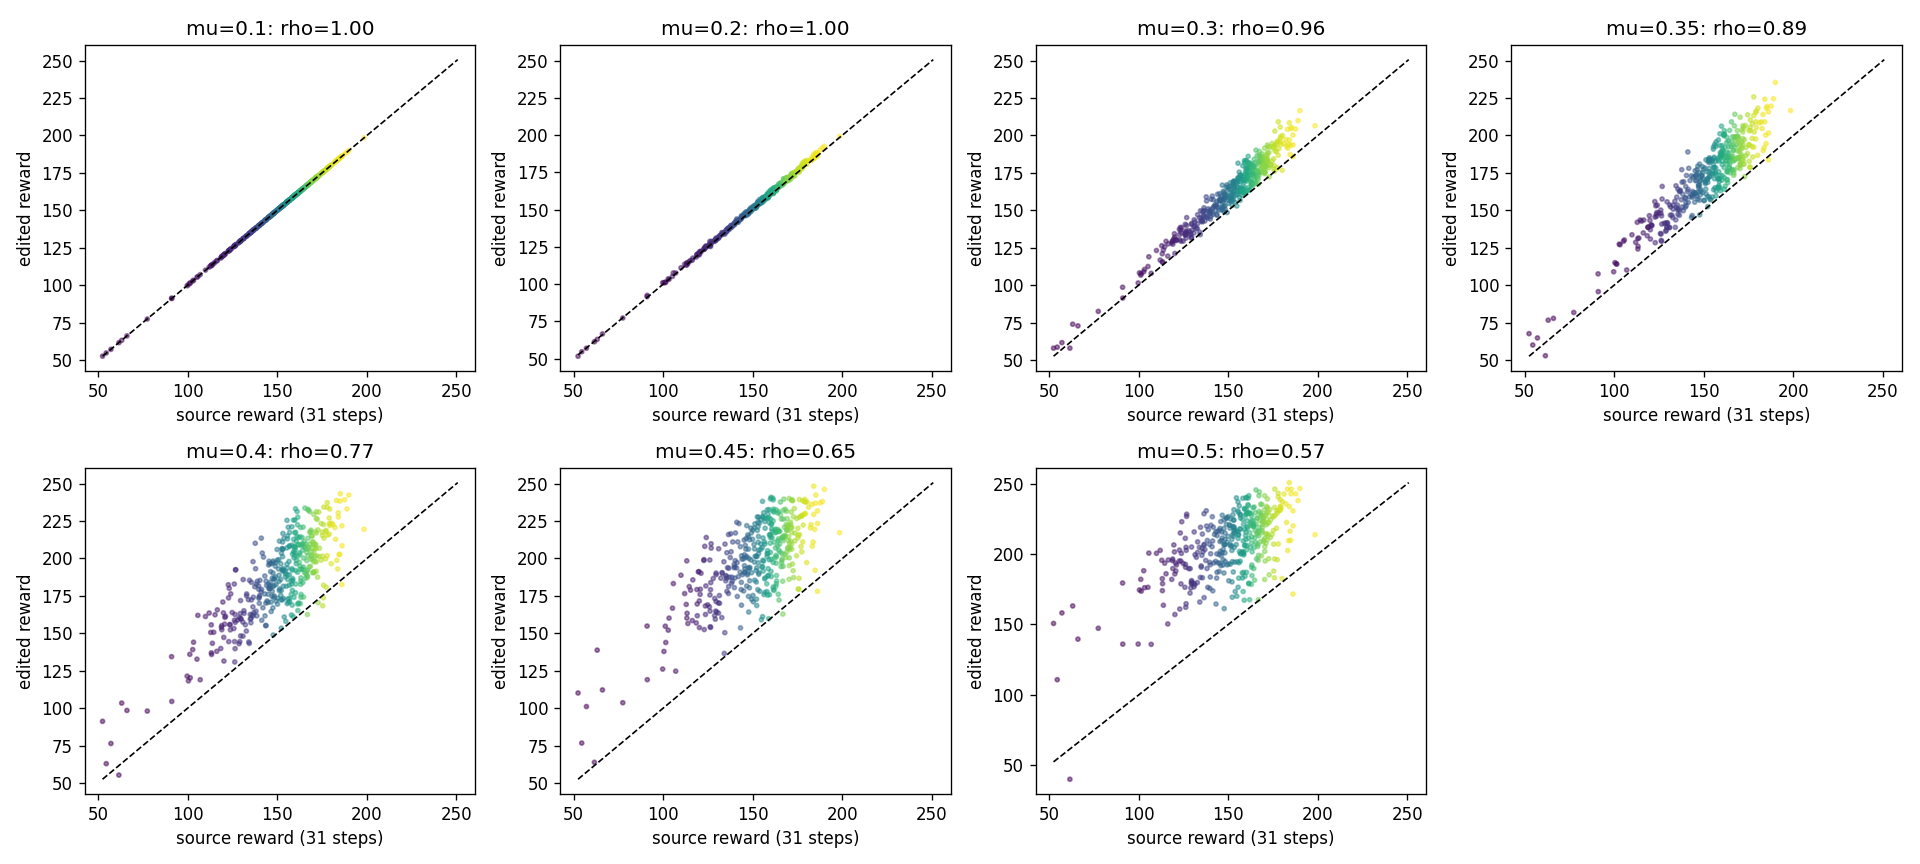
\includegraphics[width=0.92\linewidth]{main_ceiling_check.png}

\raggedright\small Edited vs source reward (31 steps) per $\mu$; colour = quality; dashed $y=x$. Edits move towards a common reward level as $\mu$ grows, so low-quality windows gain more. This is why reward gain alone cannot measure the best $\mu$.
\end{frame}

\begin{frame}{H2 scorecard (main study)}
\small
\renewcommand{\arraystretch}{1.2}
\begin{tabularx}{\linewidth}{@{}p{0.24\linewidth}Yp{0.16\linewidth}@{}}
\toprule
claim & evidence & result\\
\midrule
\hyp{H2a} more support $\Rightarrow$ higher $\mu$ & $\mu^{\text{safe}}$: $+0.18$ $[0.14,0.23]$; support predicts physics error at every $\mu$, two independent support metrics ($\rho$ $-0.13$ to $-0.36$) & \yes{} (safety)\\
 & reward-optimal $\mu^*$: $+0.06$ $[0.03,0.09]$, below the 0.1 size rule & weak\\
\hyp{H2b} higher quality $\Rightarrow$ lower $\mu$ & $\beta_Q\approx0$ for $\mu^*$ and $\mu^{\text{safe}}$; only $\mu_{90}$: $-0.05$. Quality predicts \emph{reward gain} ($\rho$ down to $-0.65$) & \nope{}\\
\hyp{H2c} support-adaptive $\mu$ helps TD3+BC & Experiment A (next slides) & running\\
\bottomrule
\end{tabularx}
\vspace{0.4em}

\textbf{One-line conclusion:} support decides how far a window can be edited before its physics breaks; quality decides how much reward the edit gains, not how strong the edit should be.
\vspace{0.3em}

\small\textbf{Side finding:} medium $\mu$ (0.3--0.45) gives the least consistent windows (half original, half generated); at $\mu=0.5$ the model regenerates a more self-consistent window but drifts further (shift 0.8--1.0 std).
\end{frame}

% =============================================================================================
\section{Experiment A}
\begin{frame}{Experiment A (H2c): design}
\small
\textbf{Question:} if $\mu$ is chosen per window from its support, does TD3+BC score higher?
\vspace{0.3em}

\begin{tabularx}{\linewidth}{lY}
\toprule
Source windows & \textbf{161{,}291} random windows from all 970{,}000 (any start, as upstream GTA), seed 0; $161{,}291\times31=5{,}000{,}021$ generated transitions. \textbf{The same windows in every condition.}\\
Support & $S_2$ (4 draws, same $\sigma$), quintiles within these windows (32{,}258 each)\\
Edit & one edit per window, $\alpha=1.3$, temperature 1\\
RL data & 1M original + 5M generated transitions per condition\\
\bottomrule
\end{tabularx}
\vspace{0.4em}

\centering
\begin{tabular}{lccccc}
\toprule
condition & \multicolumn{5}{c}{$\mu$ for support quintile (lowest $\to$ highest)}\\
\midrule
\texttt{none} & \multicolumn{5}{c}{original data only}\\
\texttt{uniform\_0.5} & 0.5 & 0.5 & 0.5 & 0.5 & 0.5\\
\texttt{uniform\_0.3} & 0.3 & 0.3 & 0.3 & 0.3 & 0.3\\
\texttt{adaptive} & 0.20 & 0.25 & 0.30 & 0.35 & 0.40\\
\texttt{inverted} & 0.40 & 0.35 & 0.30 & 0.25 & 0.20\\
\bottomrule
\end{tabular}

\raggedright\scriptsize \texttt{adaptive} follows the $\mu^{\text{safe}}$ curve (0.20$\to$0.34). \texttt{uniform\_0.3} has the same average $\mu$ but no targeting; \texttt{inverted} has the same $\mu$ values in the wrong order. \texttt{uniform\_0.5} is the paper's setting.
\end{frame}

\begin{frame}{Experiment A: training and decision rule}
\small
\begin{tabularx}{\linewidth}{lY}
\toprule
Algorithm & TD3+BC, CORL implementation (as the paper, App.~C.2)\\
Networks & actor and two critics, 2 hidden layers $\times$ 256, Adam lr $3\cdot10^{-4}$\\
TD3+BC & $\gamma=0.99$, $\tau=0.005$, policy noise 0.2, clip 0.5, actor delay 2, $\alpha_{\text{BC}}=2.5$, states normalised over the training set\\
Batch, steps & \textbf{1{,}024} (paper App.~C.3), \textbf{1M} gradient steps\\
Evaluation & every 10k steps, 10 episodes, D4RL normalised score; \textbf{final score} = mean of the last 5 evaluations (960k--1M)\\
Seeds & 0, 1, 2 for each of the 5 conditions (15 runs)\\
Reference & paper Table~1: TD3+BC 48.4 (no augmentation), 57.8 (GTA); Table~29: $\mu=0.5,\alpha=1.3$: 57.9\\
\bottomrule
\end{tabularx}
\vspace{0.4em}

\textbf{Decision rule (fixed before results):} H2c \yes{} if \texttt{adaptive} beats \textbf{both} \texttt{uniform\_0.3} and \texttt{inverted} (Welch $t$-test, $p<0.05$). Comparisons with \texttt{uniform\_0.5} and \texttt{none} are reported but not part of the rule.
\vspace{0.3em}

\scriptsize Smoke test (3{,}000 windows, \texttt{adaptive}): simulator reward 161.4 vs 148.8 for the sources, mean physics error 0.0088.
\end{frame}

\begin{frame}{Experiment A: status and results}
\textbf{Status:} running (generation of the 4 datasets, then 3 rounds of 5 parallel TD3+BC runs; $\approx7$--8 h in total).
\vspace{0.5em}

\centering\small
\begin{tabular}{@{}lccc@{}}
\toprule
condition & final score (mean $\pm$ std, 3 seeds) & physics error of its data & mean $\mu$\\
\midrule
\texttt{none} & [\ \ ] & -- & --\\
\texttt{uniform\_0.5} & [\ \ ] & [\ \ ] & 0.50\\
\texttt{uniform\_0.3} & [\ \ ] & [\ \ ] & 0.30\\
\texttt{adaptive} & [\ \ ] & [\ \ ] & 0.30\\
\texttt{inverted} & [\ \ ] & [\ \ ] & 0.30\\
\bottomrule
\end{tabular}
\vspace{0.5em}

\raggedright\small Filled from \texttt{outputs/h2\_rl/rl\_summary.md} and \texttt{figures/rl\_results.png} when the runs finish.
With 3 seeds, differences below $\approx1$ point are unlikely to be significant; seeds 3--4 can be added without rerunning anything.
\end{frame}

% =============================================================================================
\section{Limitations}
\begin{frame}{Limitations and threats to validity}
\footnotesize
\begin{itemize}
\item \textbf{One dataset}, one behaviour policy: support varies only moderately (relative spread 0.52). Results may differ on mixed datasets (e.g.\ medium-replay).
\item \textbf{Proxy outcomes}: H2a/H2b are tested on data quality (simulator reward, physics error), not on RL performance. H2c (Experiment A) is the RL test.
\item \textbf{Threshold dependence}: $\mu^*$ and $\mu^{\text{safe}}$ depend on $\theta$. Reported at 0.0085 (paper's mean) and 0.017; direction unchanged.
\item \textbf{Analysis choices from the pilot}: $\mu\le0.5$ and $\theta=0.0085$ were fixed after the pilot (different windows), then tested in the main run. $\mu^{\text{safe}}$ was added after the first main analysis: \textbf{exploratory}.
\item \textbf{Grid ceiling}: $\mu^*$ is capped at 0.5 (70\% of windows sit there).
\item \textbf{Two noise draws} per edit; per-window metrics are noisy (averaged over 400 windows in all tests).
\item \textbf{Guidance} at $w=0$ instead of the paper's $w=2$; condition dropout active during sampling (upstream).
\item Quality and support are correlated ($\rho\approx0.42$); the stratified design and the regression with both terms separate them.
\end{itemize}
\end{frame}

\begin{frame}{Reproducibility}
\scriptsize
Repository branch \texttt{dev-karan}; environment and setup in \texttt{README.md}.
\vspace{0.3em}

\begin{tabularx}{\linewidth}{lY}
\toprule
command & produces\\
\midrule
\texttt{python scripts/gta\_edit\_demo.py --ckpt <1M checkpoint>} & 4-window demo (\texttt{outputs/gta\_demo/})\\
\texttt{python scripts/h2\_run.py pool} & pool of 20k windows with $Q$, $S_1$, $S_2$, $S_3$ (\texttt{outputs/h2/pool.csv})\\
\texttt{python scripts/h2\_run.py sweep} & 400 windows $\times$ 8 $\mu$ $\times$ 2 draws, simulator metrics (\texttt{sweep\_parts/})\\
\texttt{python scripts/h2\_run.py analyze --max\_mu 0.5 --thr 0.0085} & figures, statistics, verdict (\texttt{summary.md})\\
\texttt{bash scripts/h2\_rl\_all.sh} & Experiment A: datasets, 15 TD3+BC runs, report (\texttt{outputs/h2\_rl/})\\
\bottomrule
\end{tabularx}
\vspace{0.4em}

Seeds: pool 0, pilot pool 1, sampling seed 0, edit seeds fixed per $(\mu,\text{draw})$; checkpoint \texttt{model-1000000.pt} (EMA weights).
Code: \texttt{src/h2/} (\texttt{common}, \texttt{quality}, \texttt{support}, \texttt{edit\_eval}, \texttt{analysis}, \texttt{render}, \texttt{rl\_data}, \texttt{rl\_train}, \texttt{rl\_report}).
\end{frame}

% =============================================================================================
\appendix
\section{Appendix}
\begin{frame}{Appendix A: columns of \texttt{pool.csv} and \texttt{selected.csv}}
\footnotesize
\begin{tabularx}{\linewidth}{lY}
\toprule
\texttt{episode}, \texttt{start} & window = steps \texttt{start}\dots\texttt{start+30} of episode \texttt{episode} (0-based)\\
\texttt{q\_return} & $q_i$: discounted ($\gamma=0.99$) reward inside the window\\
\texttt{rtg} & discounted return-to-go from \texttt{start} to the episode end (the model's condition before $\times0.01\times\alpha$)\\
\texttt{s1\_dist} & median over the 31 steps of the distance to the 20th nearest other-episode transition (lower = more support)\\
\texttt{s2\_err\_sigma0.16/0.5/2.4} & one-step denoising error at each $\sigma$ (mean of 4 draws)\\
\texttt{s2\_score} & $-$mean of the $z$-scored log errors (higher = more support)\\
\texttt{s3\_loglik} & exact log-likelihood (100 windows; empty otherwise)\\
\texttt{Q}, \texttt{S1}, \texttt{S2} & percentile ranks in the pool (higher = better quality / more support)\\
\texttt{q\_bin}, \texttt{s\_bin} & quintile (0--4) of \texttt{Q} and of the support used for sampling (selected.csv)\\
\texttt{window} & index 0--399 of the selected window (selected.csv)\\
\texttt{src\_oracle\_r} & simulator reward of the unedited window (selected.csv)\\
\bottomrule
\end{tabularx}
\end{frame}

\begin{frame}{Appendix B: columns of \texttt{sweep.csv}, \texttt{best\_mu.csv}, \texttt{metrics.csv}}
\footnotesize
\begin{tabularx}{\linewidth}{lY}
\toprule
\texttt{mu}, \texttt{draw} & editing strength and noise draw (0 or 1) of this edit; in \texttt{metrics.csv} \texttt{mu}=0 is the source\\
\texttt{gen\_r}, \texttt{oracle\_r} & model-written vs simulator reward, summed over 31 steps\\
\texttt{dyn\_mse}, \texttt{shift} & physics error and distance from the source (dataset-std units)\\
\texttt{gain\_abs}, \texttt{gain\_rel} & \texttt{oracle\_r}$-$\texttt{src\_oracle\_r}, and that divided by $\max(|\texttt{src\_oracle\_r}|,1)$\\
\texttt{S} & the support column used in the analysis (here \texttt{S2})\\
\texttt{mu\_star}, \texttt{mu90}, \texttt{mu\_safe} & per-window outcomes (definitions on the ``best $\mu$'' slide), after averaging the 2 draws\\
\texttt{quadrant} & \texttt{Q} and \texttt{S} split at 0.5 (``high Q / low S'' etc.)\\
\bottomrule
\end{tabularx}
\vspace{0.5em}

\textbf{Experiment A files:} \texttt{data/sources.npz} (161{,}291 windows, \texttt{s2\_score}, \texttt{s\_bin}); \texttt{data/<condition>.npz} (5{,}000{,}021 transitions, per-window \texttt{mu}, 5{,}000-window quality check \texttt{check\_*}); \texttt{runs/<condition>\_seed<k>/evals.csv} (\texttt{step}, \texttt{d4rl\_score}).
\end{frame}

\begin{frame}{Appendix C: pilot vs main study at a glance}
\centering
\footnotesize
\begin{tabular}{@{}lll@{}}
\toprule
 & pilot & main\\
\midrule
pool & 500 (seed 1) & 20{,}000 (seed 0)\\
support for sampling & $S_1$ (kNN) & $S_2$ (model)\\
selected windows & 184 (8 per cell, sparse corner) & 400 (16 per cell, full)\\
$\mu$ grid & 8 values incl.\ 0.75 & same; analysis uses $\mu\le0.5$\\
threshold $\theta$ & 0.017, then 0.0085 & 0.0085 (fixed)\\
support $\to$ physics error, $\mu\le0.45$ & $\rho$ $-0.27$ to $-0.40$ & $\rho$ $-0.18$ to $-0.36$\\
$\beta_S$ for $\mu^*$ ($\mu\le0.5$, $\theta=0.0085$) & $+0.087$ $[0.037,0.141]$ & $+0.059$ $[0.030,0.090]$\\
$\beta_Q$ for $\mu^*$ (same) & $-0.012$ $[-0.045,0.018]$ & $-0.001$ $[-0.025,0.022]$\\
\bottomrule
\end{tabular}
\vspace{0.6em}

\raggedright\small The pilot's support effect replicated in the main run with a different support metric and different windows (smaller, still significant).
\end{frame}

\end{document}
